\documentclass{ximera}

\input{../../preamble.tex}

\author{Bobby Ramsey}

\begin{document}




Given a right triangle with angles, measuring $u$ and $v$, and side lengths as marked:
\begin{image}[2in]
  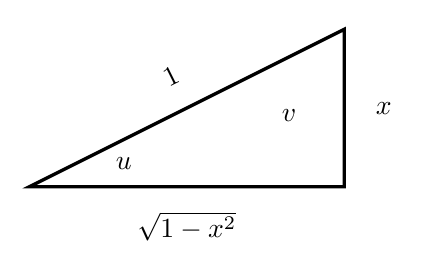
\begin{tikzpicture}
    \coordinate (C) at (0,2);
    \coordinate (D) at (4,2);
    \coordinate (E) at (4,4);
    \tkzMarkRightAngle(C,D,E)
    \tkzMarkAngle(D,C,E)
    \tkzMarkAngle(C,E,D)
    \node at (2,2-.5) {$\sqrt{1-x^2}$};
    \node at (4+.5,3) {$x$};
    \node[rotate=26.5] at (2-.2,3+.4) {$1$};
%    \draw[decoration={brace,mirror,raise=.2cm},decorate,thin] (0,2)--(4,2);
%    \draw[decoration={brace,mirror,raise=.2cm},decorate,thin] (4,2)--(4,4);
%    \draw[decoration={brace,raise=.2cm},decorate,thin] (0,2)--(4,4);
    \draw[very thick] (D)--(E)--(C)--cycle;
    \node at (1.2,2.3) {$u$};
    \node at (3.3, 2.9){$v$};
  \end{tikzpicture}
\end{image}

\begin{exercise}
	What is the sum of the two angles: $u + v$?
	\[ u + v = \answer{\frac{\pi}{2}} \]
	\begin{hint}
		Remember that $u$ and $v$ are two angles in a right triangle.  Be sure to use radians.
	\end{hint}
	\begin{exercise}
		In terms of $x$, what is $\sin(u)$?
		\[ \sin(u) = \answer{x} \]
		\begin{hint}
			Think: SOH-CAH-TOA
		\end{hint}
		\begin{exercise}
			In terms of $x$, what is $\cos(v)$?
			\[ \cos(v) = \answer{x} \]
			\begin{hint}
				Think: SOH-CAH-TOA
			\end{hint}
			\begin{exercise}
				What are $\sin^{-1}(x)$ and $\cos^{-1}(x)$ in terms of $u$ and $v$?
				\begin{align*}
					\sin^{-1}(x) &= \answer{u} \\ \\
					\cos^{-1}(x) &= \answer{v}
				\end{align*}
				\begin{hint}
					Remember that you've already found that $\sin(u) = x$, and $\cos(v) = x$.
				\end{hint}
				\begin{exercise}
					What is $\sin^{-1}(x) + \cos^{-1}(x)$?
					\[  \sin^{-1}(x) + \cos^{-1}(x) = \answer{\frac{\pi}{2}} \]
					\begin{hint}
						Remember from above what you found $u+v$ equaled?
					\end{hint}
				\end{exercise}
			\end{exercise}
		\end{exercise}
	\end{exercise}
\end{exercise}
\end{document}
